\section{Appendices}
\begin{appendices}

\section{GMM model tuning}

% Preamble:
% \usepackage{graphicx}
% \usepackage{subcaption}

\begin{figure}[htbp]
  \centering

  \begin{subfigure}[t]{\textwidth}
    \centering
    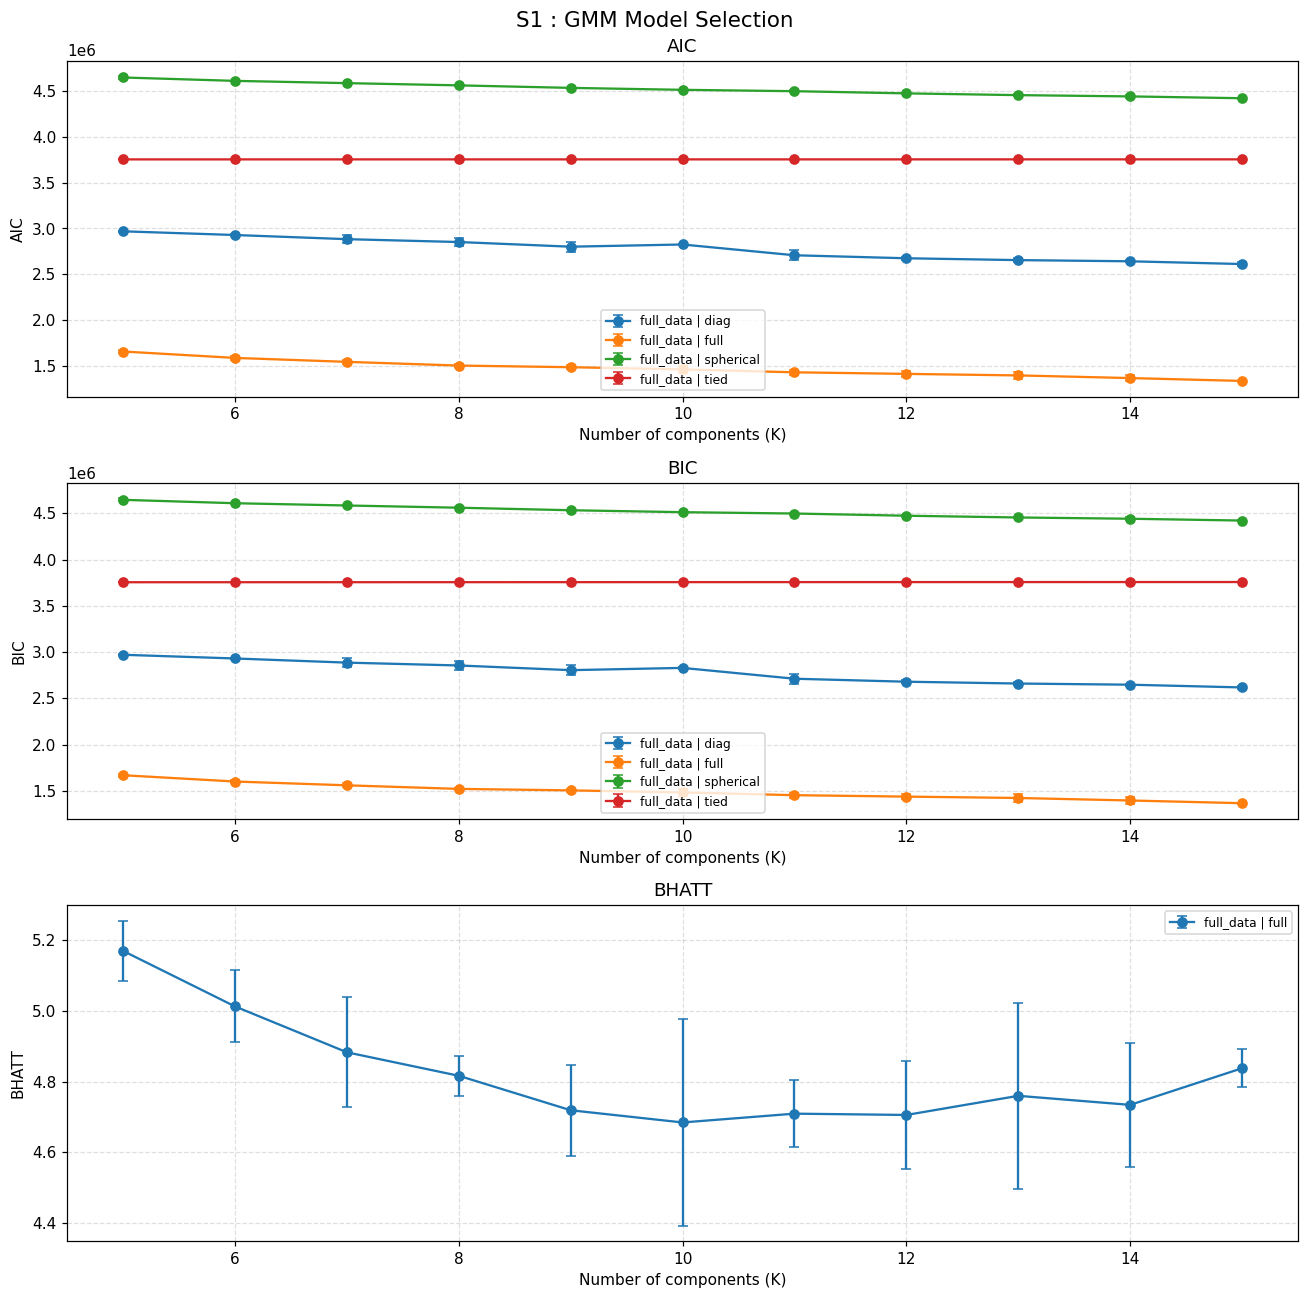
\includegraphics[width=\textwidth]{figures/appendix/S1_gmm_model_selection.png}
    \caption{S1: Model selection}
    \label{fig:s1_sel}
  \end{subfigure}

  \medskip

  \begin{subfigure}[t]{\textwidth}
    \centering
    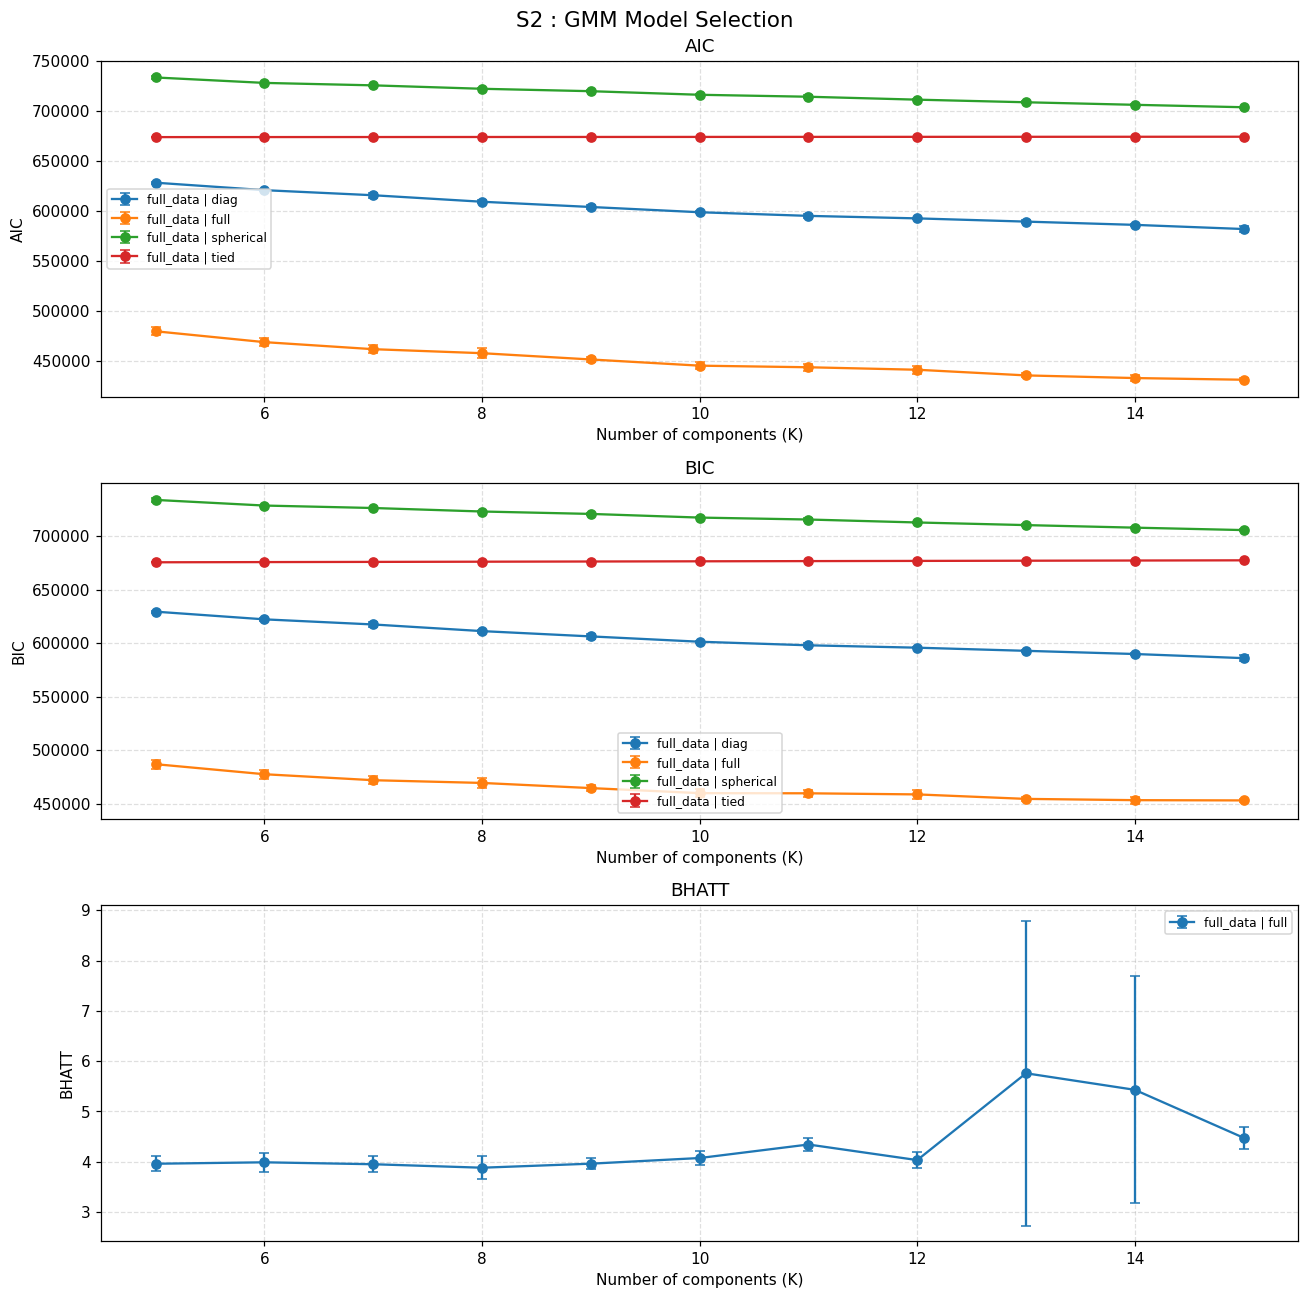
\includegraphics[width=\textwidth]{figures/appendix/S2_gmm_model_selection.png}
    \caption{S2: Model selection}
    \label{fig:s2_sel}
  \end{subfigure}

  \label{fig:two-rows}
\end{figure}

\section{Cluster properties of S2 and S3}

% Preamble:
% \usepackage{graphicx}
% \usepackage{subcaption}

\begin{figure}[htbp]
  \centering

  % --- Top Left ---
  \begin{subfigure}[t]{0.48\textwidth}
    \centering
    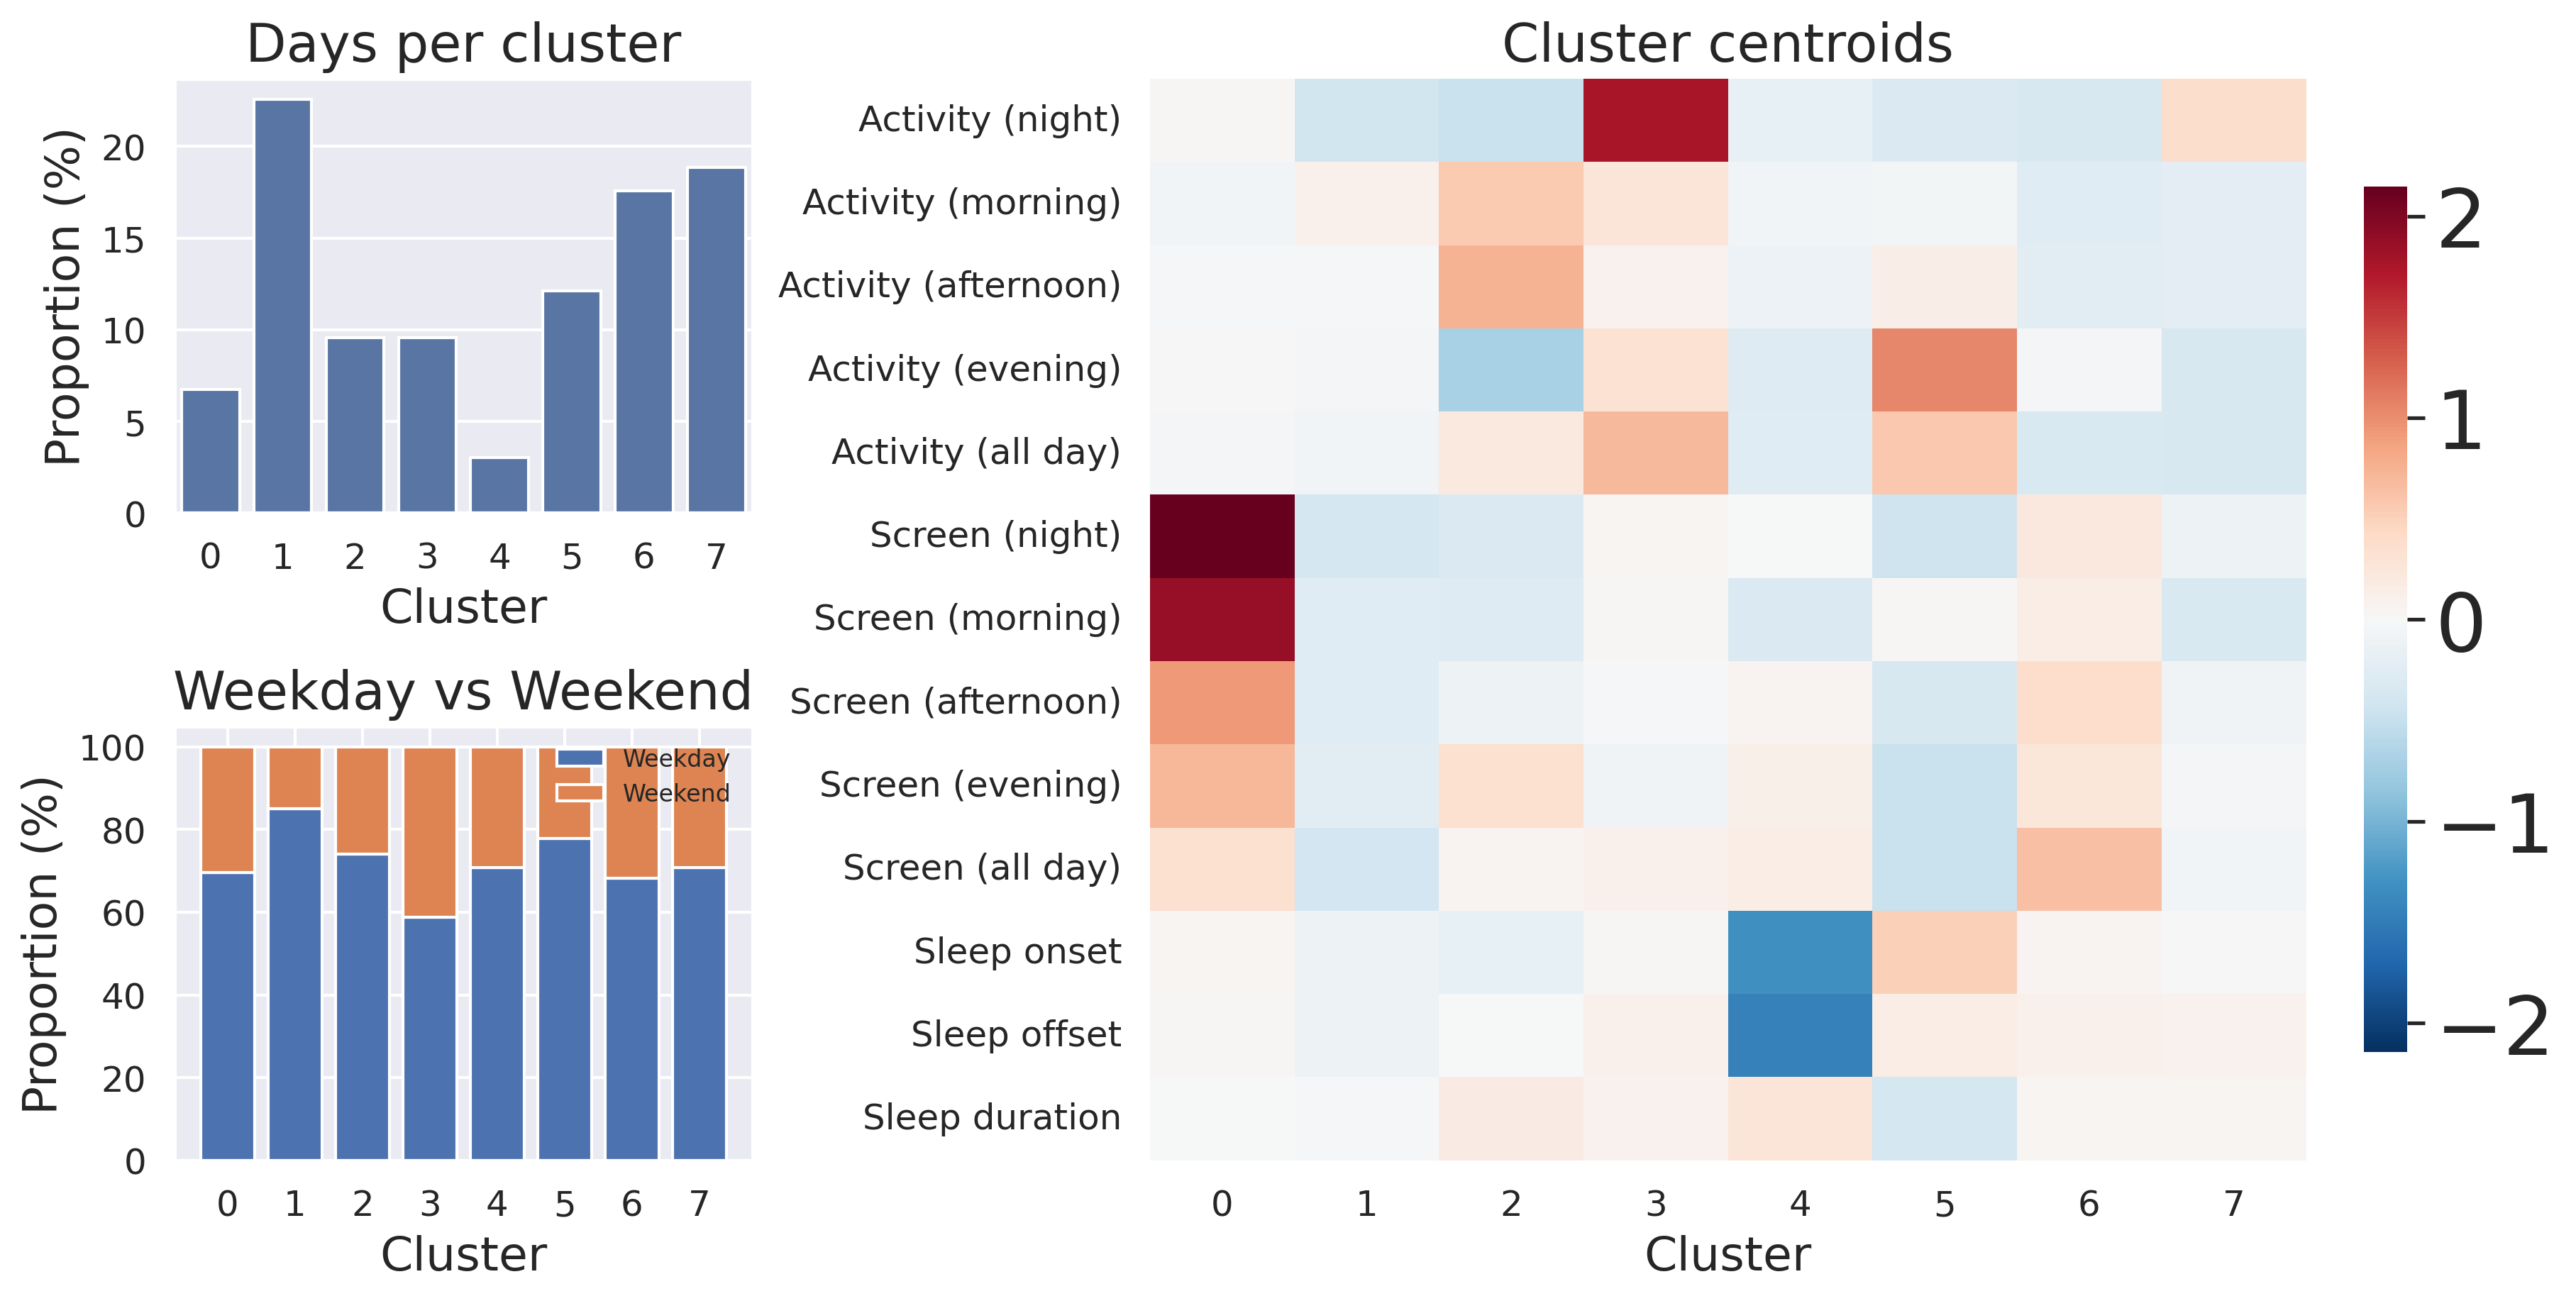
\includegraphics[width=\textwidth]{figures/appendix/globem_INS-W_1_summary.png}
    \caption{S3: Wave 1}
    \label{fig:top-left}
  \end{subfigure}
  \hfill
  % --- Top Right ---
  \begin{subfigure}[t]{0.48\textwidth}
    \centering
    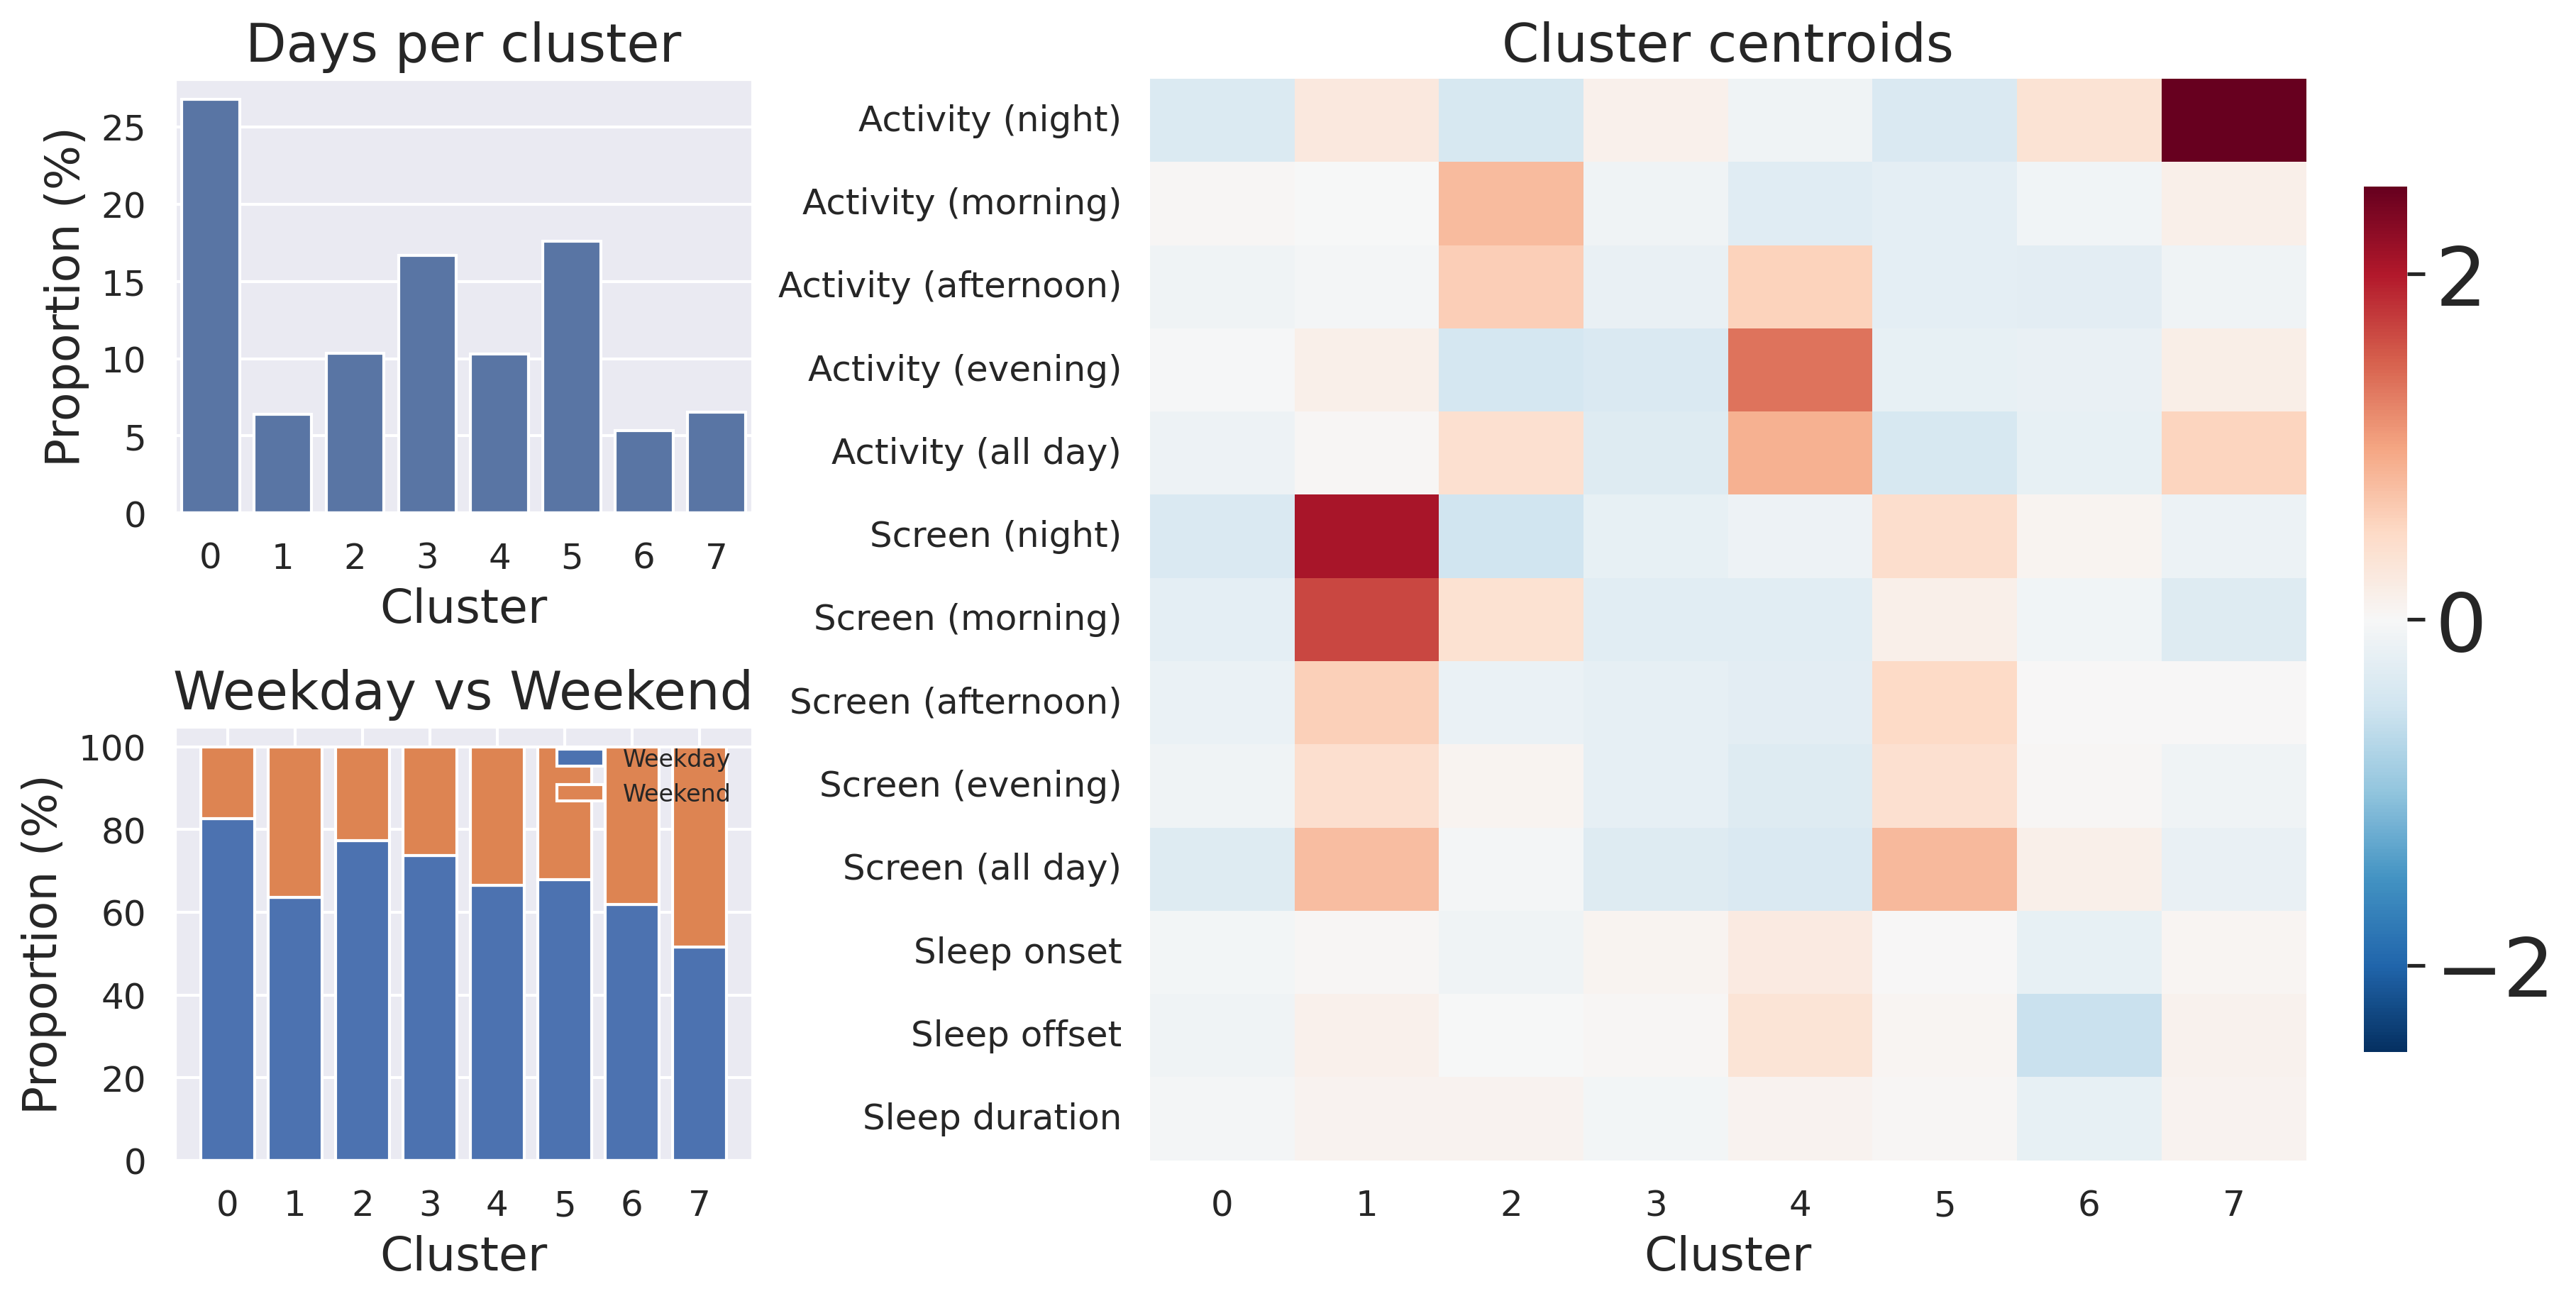
\includegraphics[width=\textwidth]{figures/appendix/globem_INS-W_2_summary.png}
    \caption{S3: Wave 2}
    \label{fig:top-right}
  \end{subfigure}

  \medskip

  % --- Bottom Left ---
  \begin{subfigure}[t]{0.48\textwidth}
    \centering
    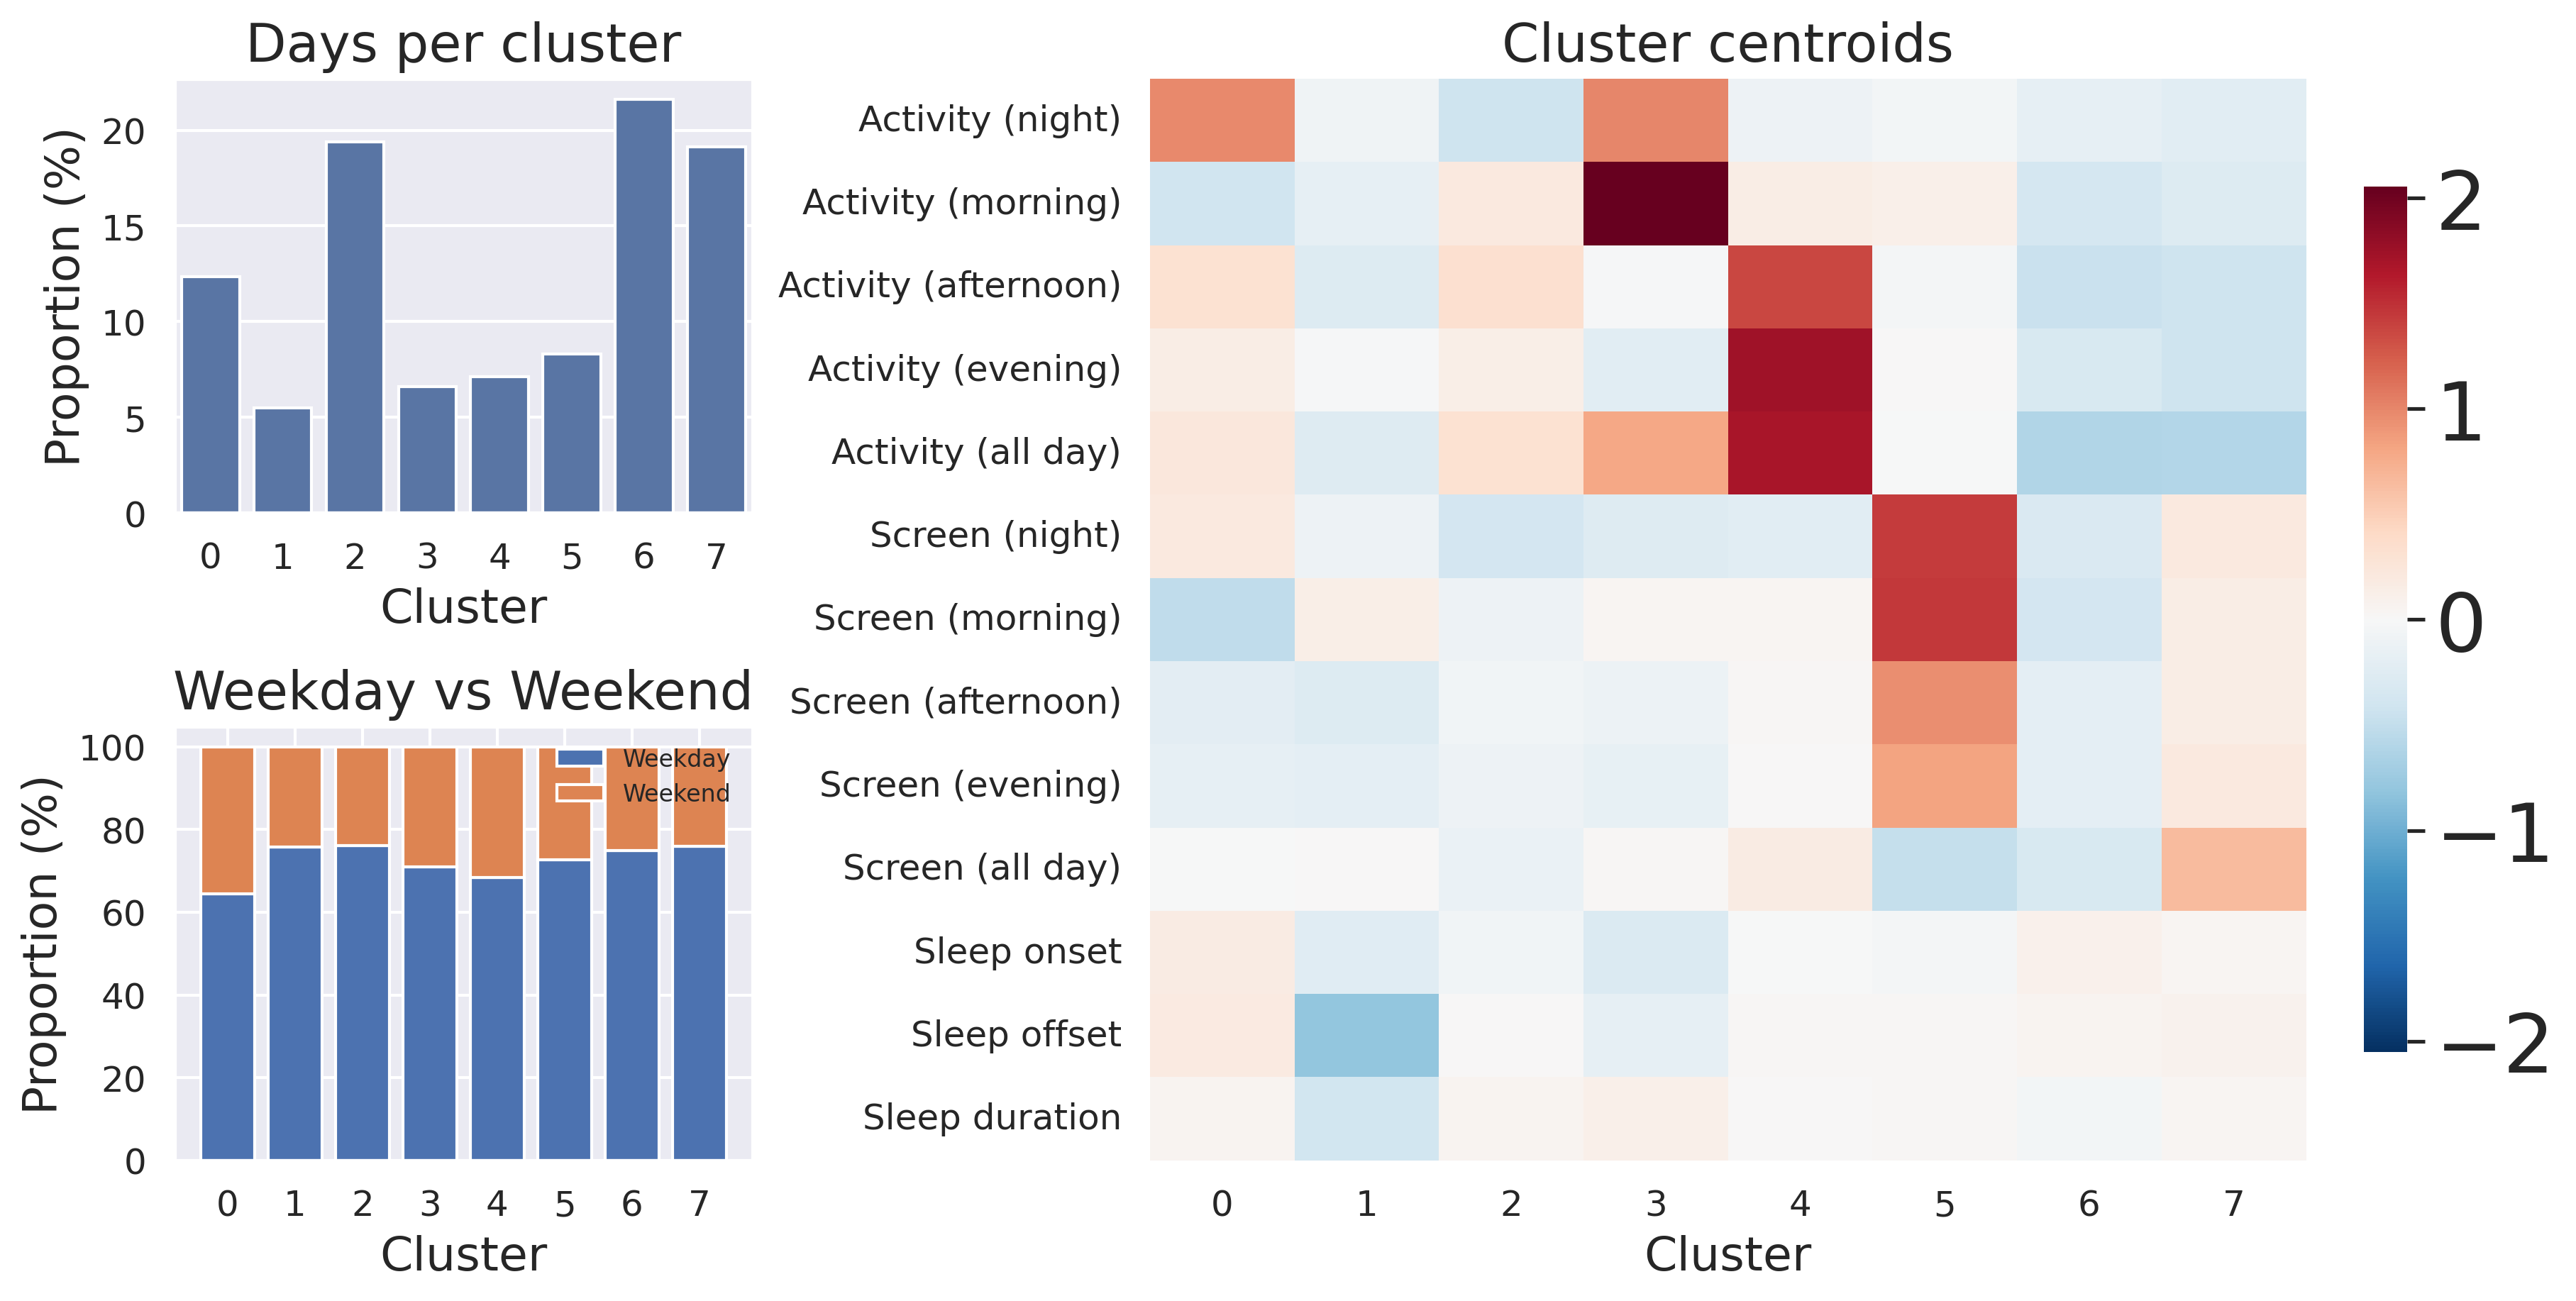
\includegraphics[width=\textwidth]{figures/appendix/globem_INS-W_3_summary.png}
    \caption{S3: Wave 3}
    \label{fig:bottom-left}
  \end{subfigure}
  \hfill
  % --- Bottom Right ---
  \begin{subfigure}[t]{0.48\textwidth}
    \centering
    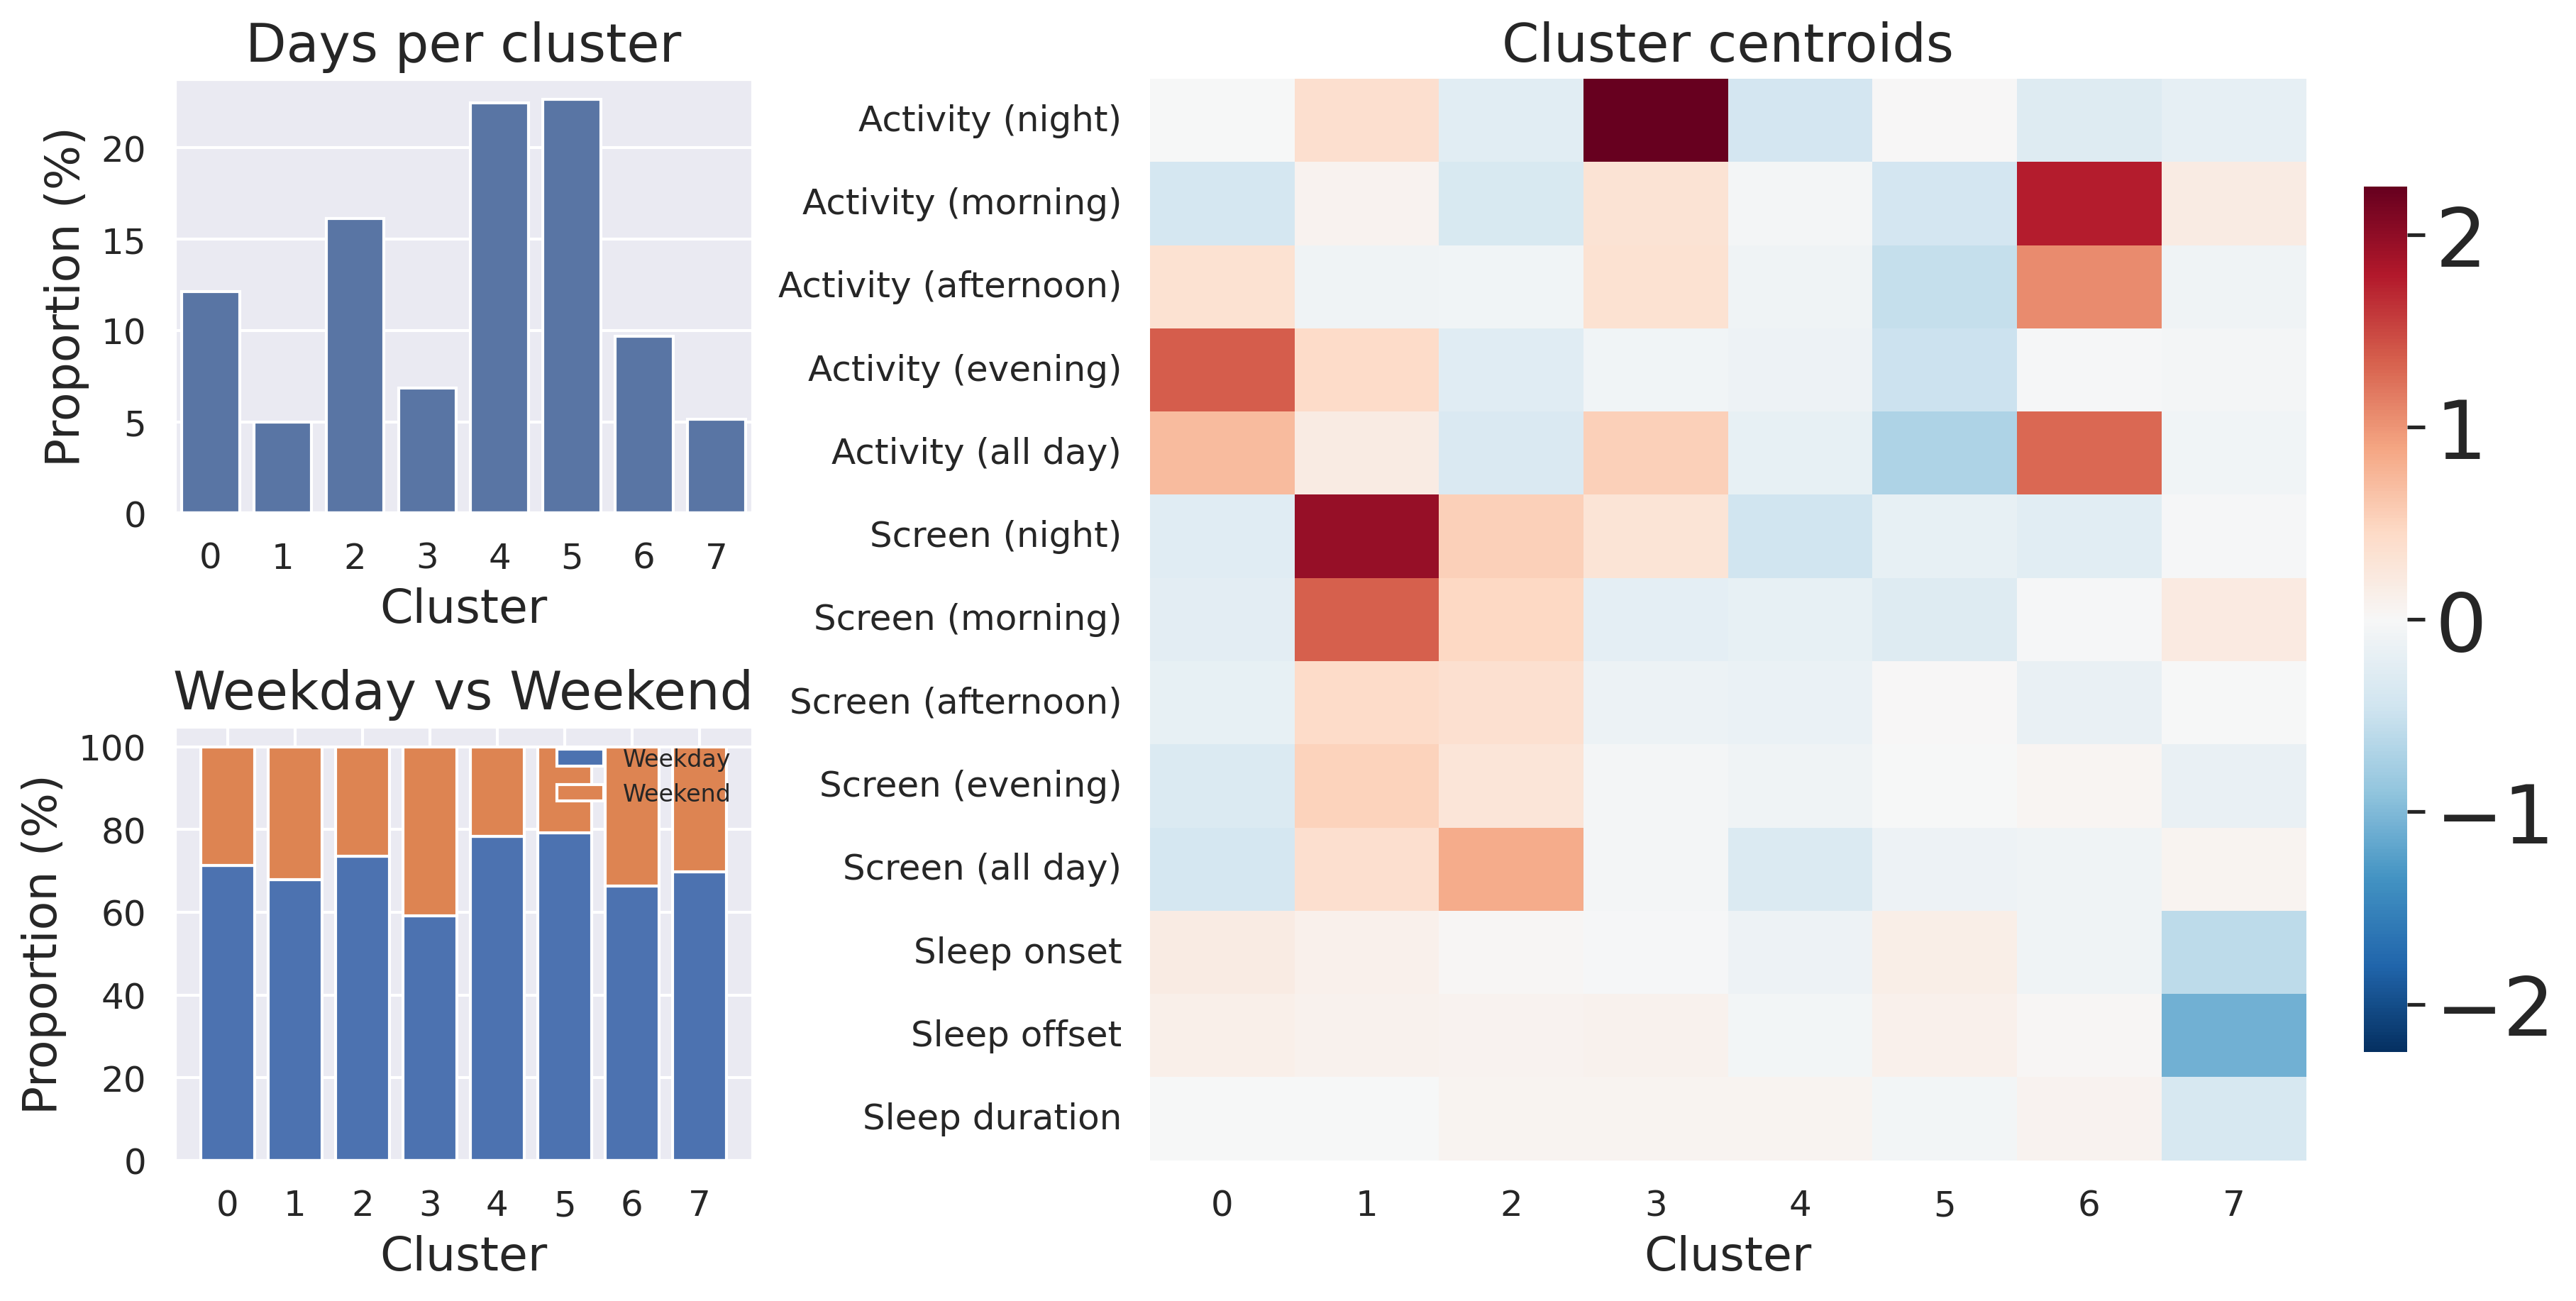
\includegraphics[width=\textwidth]{figures/appendix/globem_INS-W_4_summary.png}
    \caption{S3: Wave 4}
    \label{fig:bottom-right}
  \end{subfigure}

  \caption{S3: Cluster characteristics in each wave}
  \label{fig:2x2}
\end{figure}


\end{appendices}